\documentclass[11pt, english, fleqn, DIV=15, headinclude, BCOR=2cm]{scrreprt}

\usepackage[
    color,
    bibatend,
]{../../header}

\graphicspath{{./}{../Figures/}}

\usepackage{needspace}

\usepackage{mathtools}
\usepackage{listings}

\lstset{
    basicstyle=\small\ttfamily,
}

\hypersetup{
    pdftitle=
}

\newcommand\mot{\textsc{mot}}

\usepackage{longtable}
\usepackage{subcaption}

\usepackage[all]{nowidow}

\subject{Lab report}
\title{Magneto-optical trap}
\subtitle{Experiment A248 -- Universität Bonn}
\author{%
    Martin Ueding \\
    \small{\href{mailto:mu@martin-ueding.de}{mu@martin-ueding.de}}
    \and
    Lino Lemmer \\
    \small{\href{mailto:l2@uni-bonn.de}{l2@uni-bonn.de}}
}

\date{\daterange{2016-04-25}{2016-04-26}}

\publishers{Tutor: Daniel Babik}

\begin{document}

\maketitle

\begin{abstract}
    In this experiment we set up a magneto-optical trap to catch rubidium
    atoms. After that we investigate basic properties of the trap and its
    components.
\end{abstract}

\tableofcontents

\chapter*{Permission to upload}

I, Martin Ueding, would like to scan and upload this lab report with your
corrections to my website \href{http://martin-ueding.de}{martin-ueding.de}.
There, the original lab report as well as the reviewed one will be licensed
under the “\href{http://creativecommons.org/licenses/by-sa/4.0/}{Creative
Commons Attribution-ShareAlike 4.0 International License}”. Is that okay with
you?

Yes $\Box$ \hspace{2cm} No $\Box$

\chapter{Theory}

\section{Optical cooling}

\subsection{Radiation pressure}

Light, being mediated by massless gauge bosons, has a quadratic dispersion
relation $E = cp$ with momentum $p = \hbar k$ and wave number $k$. An atom
which absorbs a photon will obtain its energy and also its momentum. While in
stimulated emission the momentum of the emitted photon points in the same
direction as the stimulating atom's momentum, spontaneous emission is isotropic
which leads to a net acceleration. This effect causes the so called radiation pressure.

\subsection{Red detuning}

To cool atoms down one has to make sure that only those atoms that move
towards the laser beam feel this pressure. This can be done using the Doppler
effect: In the rest system of the atom, that flies towards the laser beam, the
photons of the laser are blue detuned, with $\nu'=\nu(1+v/c)$, where $v$ is
the velocity of the atom. To get those atoms on resonance again one has to
detune the laser to the red.

\subsection{Optical molasses}

The force of a laser with intensity $I$ and detuning $\delta =
\omega_\text{laser}-\omega_\text{res}$ on an atom can be expressed as
\[
    F_\text{radiation} = \frac{\hbar k\Gamma}2\cdot\frac{I/I_\text{S}}{\del{2\frac{\delta -
    kv}\Gamma}^2 + 1 + I/I_\text{S}}\, ,
\]
where $k$ denotes the wave vector of the photons, $\Gamma$ the decay rate of the
excited state and $I_\text{S}$ the saturation intensity. This force is non zero
at $v=0$ as we would need to cool down. To solve this one uses two
counterpropagating laser beams with the same detuning. For small velocities
this gives a frictional force:
\[
    F_\text{count} = \frac{8\hbar k^2\delta}{\Gamma}
    \frac{I/I_\text{S}}{\del{\del{2\delta/\Gamma}^2 + 1 + I/I_\text{S}}^2}
    \cdot v \underset{\delta<0}{=} -\alpha\cdot v \, .
\]
Applying three orthogonal pairs of lasers gives an effective deacceleration of
atoms and with this a cooling. This setup is known as \emph{optical molasses}.
This process is limited by heating due to spontaneous emission. This leads to
the so called \emph{Doppler limit}:
\[
    T_\text{Doppler} = \frac{\hbar \Gamma}{2k_\text{B}} \, .
\]

\section{Magneto-optical trap}

Since the forces in the optical molasses are independent of space, the atoms
have the possibility to diffuse out of the cooling area. Due to collisions
those atoms get heated up again. We need an additional force that keeps the
atoms inside that area. One possibility is to use a \emph{magneto optical trap}
(\mot).

To simplify the working principle we consider a two level system with one
possible transition ($F=0 \to F=1$). Also we add a 1-dimensional linear
increasing magnetic field (w.l.o.g.) along the $z$ axis, which is zero at
$z=0$. Due to the Zeeman effect we get a space-dependent energy splitting of
the three possible $F=1$ configurations, which causes a lowering of the $m=1$
state's energy for $z<0$ and a lowering of the $m=-1$ level for $z>0$ (see
Figure~\ref{fig:mot-principle}).

Now we add two counterpropagating laser beams with detuning $\delta<0$. If now
the laser beam propagating in positive $z$ direction has a $\sigma^+$ helicity
and the counterpropagating beam has a $\sigma^-$ helicity, atoms which are
located at $z<0$ have a higher possibility to absorb $\sigma^+$ photons and
hence get pushed back to $z=0$. For atoms at $z>0$ it is the other way around.
There the absorption of a $\sigma^-$ photon is more likely, so that they 
also get pushed back to $z=0$.

While in reality the energy levels are way more complex the working principle
remains the same.

\begin{figure}
    \centering
    \includegraphics[width=.5\textwidth]{mot-principle}
    \caption{%
        Energy levels and transitions in a spatially varying magnetic field.
    }
    \label{fig:mot-principle}
\end{figure}

\section{Rubidium}

Natural rubidium consists about \SI{72}{\percent} of ${}^{85}\text{Ru}$ and
\SI{28}{\percent} of ${}^{87}\text{Ru}$. In our \mot{} we use the former.
Part of its hyperfine level scheme is shown in Figure~\ref{fig:rubidium85}. To
create a quasi two level system we use the closed $F=3 \to F'=4$ transition.
Since this is not a real two level system there is a finite probability for the
transition from $F'=4$ to $F=2$. In this state the atom can not be excited by
the cooling laser. Therefor it is called \emph{dark state}. To solve this
problem a second laser, the \emph{pumping laser} excites the atoms in the dark
state to the $F'=3$ state, from where it can decay into the cooling ground
state $F=3$ again and with this get the atom back in the cooling cycle

\begin{figure}
    \centering
    \includegraphics[width=.5\textwidth]{rubidium85}
    \caption{%
        Part of the ${}^{85}\text{Ru}$ level scheme. The colored transitions
        are the ones used in this experiment. The cooling beam uses the red
        transition while the blue transition is needed for the repumping.
    }
    \label{fig:rubidium85}
\end{figure}

\section{Doppler-free spectroscopy}

Since the Doppler broadening of spectral lines at room temperature is orders of
magnitude bigger than the natural linewidth, lines which lie close together can
not be resolved. To nevertheless investigate those lines one has to use
Doppler-free spectroscopy.

\subsection{Pump and probe beam}

For this two counterpropagating laser beams of same frequency are needed, a
\emph{pump beam} and a \emph{probe beam} with lower intensity. The absorption
of the probe beam gets recorded. For a simple understanding again consider a
two level system with ground state $\ket{g}$, excited state $\ket{e}$ and
energy difference of $\hbar\omega_0$. If the lasers both have the frequency
$\omega_0$ atoms with $v\neq0$ along the laser's direction will be out of
resonance due to the Doppler effect. Those atoms with $v\approx 0$ will be
excited by the pump beam and hence the absorption of the probe beam is very
low. If the lasers are detuned to the red from the resonance frequency the pump
beam and the probe beam excite oncoming atoms with respect to their own
propagation direction. Therefor the absorption of the probe beam is high.
The same holds for blue detuned lasers. This leads to a transmission spectrum as
in Figure~\ref{fig:doppler-free-2-level}.

In reality there will be more levels, which makes the absorption spectrum more
complex. Take for example a system with one ground level and two excited level
with excitation energy $\hbar\omega_1$ and $\hbar\omega_2$ respectively. When
we apply the same method as above it can happen, that the pump beam is on
resonance with one of the excited levels and the probe beam with the other.
This leads to a so called \emph{cross over peak} at $\omega_\text{probe} =
\frac{\omega_1+\omega_2}2$ (see
Figure~\ref{fig:doppler-free-3-level}).

\begin{figure}
    \begin{subfigure}{.5\textwidth}
        \centering
        \includegraphics[width=.8\linewidth]{doppler-free-2-level}
        \caption{%
            Two level system.
        }
        \label{fig:doppler-free-2-level}
    \end{subfigure}
    \hfill
    \begin{subfigure}{.5\textwidth}
        \centering
        \includegraphics[width=.8\linewidth]{doppler-free-3-level}
        \caption{%
            Three level system.
        }
        \label{fig:doppler-free-3-level}
    \end{subfigure}
    \caption{%
        Transmission spectra in Doppler-free spectroscopy.
    }
\end{figure}

\subsection{Groups of atoms with similar velocity}

\subsection{Lamp dip}

\subsection{Crossover resonance}

\subsection{Rubidium spectrum}

\section{Polarization spectroscopy}

\subsection{Circularly polarized light}

\subsection{Anisotropic pumping}

\subsection{Birefringence}

\subsection{Detection of tilt}

\subsection{Dispersion}

\subsection{Kramers-Kronig relation}

\section{Equipment}

\subsection{Anti-Helmholtz coils}

\subsection{Vacuum chamber}

\subsection{Laser system}

\subsection{Diode lasers}

\chapter{Conduction}

\section{Apparatus}

\section{Setup and calibration}

First we have to lock the cooling laser to the right transition. For this we
tune the laser roughly to the wanted frequency. The lock box gets a triangular
signal from a function generator, changes its amplitude and offset and gives it
to the piezo which controls the gratings position. The Doppler-free spectrum of
the $F=3$ ground state of ${}^{85}\text{Ru}$ is shown in
Figure~\ref{fig:doppler-free-cooling}. From there we choose the right line,
zoom in and lock the laser to a frequency a bit below it. 

\begin{figure}
    \centering
    \includegraphics{doppler-free-cooling}
    \caption{%
        Doppler-free spectrum of the ${}^{85}\text{Ru}$ $F=3 \to F'=2,3,4$
        lines. The time is related to the lasing frequency via the triangular
        voltage applied to the piezo.
    }
    \label{fig:doppler-free-cooling}
\end{figure}

For the pumping laser we repeat the last steps. The Doppler-free spectrum of the
$F=2$ ground state of ${}^{85}\text{Ru}$ is shown in
Figure~\ref{fig:doppler-free-pumping}. The lines are so close together, that we
can not distinguish between them. Instead of trying to lock we quasi-lock by
zooming in far to the place where we expect the right transition to be.

\begin{figure}
    \centering
    \includegraphics{doppler-free-pumping}
    \caption{%
        Doppler-free spectrum of the ${}^{85}\text{Ru}$ $F=2 \to F'=1,2,3$
        lines. The time is related to the lasing frequency via the triangular
        voltage applied to the piezo. Since one can not distinguish between
        lines, the labels are only rough estimates. 
    }
    \label{fig:doppler-free-pumping}
\end{figure}

Now we check if enough light is passing through the fiber. With the
powermeter we measure a total power of \SI{16.8}{\milli\watt}. Then be block
the path of the pumping laser and measure again. Now we get
\SI{14.1}{\milli\watt}. The instruction states the cooling laser needs to be at
least \SI{5}{\milli\watt} and the pumping laser \SI{1}{\milli\watt}, which both
is clearly the case for our setup.

After that we have to adjust the polarizing beam splitter and the mirrors. For
that we first check, if the first \textsc{pbs} and the bottom elevator mirrors
are hit nicely by the beam. As this is the case we modify the bottom
$z$-mirror's orientation such that the beam passes through the center of the
vacuum chamber. Then we adjust the top mirror such that the beams overlap
perfectly. This can be checked with the help of a camera, which is still
sensitive to the beam's wavelength.

Before we adjust the transversal ($x$ and $y$) beams we try to get equal light
power to each axis. So we measure the fiber power again, which is
\SI{15.1}{\milli\watt} and set the $z$-axis power to to \SI{5.0}{\milli\watt}
by rotating the $\lambda/2$ plate behind the fiber. Against our expectations we
then have no power on the transversal elevator. We try it the other way around
and adjust the $\lambda/2$ plate again until we have \SI{8.8}{\milli\watt} on
the elevator and \SI{4.8}{\milli\watt} on the $z$-axis.

After measuring the beam power directly in front of the vacuum chamber we
realize that we incur loss on all the mirrors and first adjust the splitting in
the transversal directions to be symmetric. There now are \SI{2.7}{\milli\watt}
on each of them. Then we adjust the initial $\lambda/2$ plate to give more
power to the transversal and less to the longitudinal direction. After that we
have \SI{3.1}{\milli\watt} behind each polarizing beam splitter.

We start to adjust the transversal mirrors. We calibrate the $y$ direction
first. When the reflected beam coincides nicely with the incident beam we move
on to the $x$ direction and repeat the procedure. 

After checking the locking of the lasers we tweak again on all the mirrors to
optimize the overlap. Now when toggling the power supply of the magnetic field,
we can see a little difference in the brightness which indicates a working
\mot. With the help of a photo diode we then adjust the laser locks to
make the \mot{} even larger.

\begin{table}
    \centering
    \begin{tabular}{SSS}
        \toprule
        {total power/\si{\nano\watt}}
        & {background/\si{\nano\watt}}
        & {power of \mot/\si{\nano\watt}} \\
        \midrule
        %< for row in power_mot_table >%
        << ' & '.join(row) >> \\
        %< endfor >%
        \bottomrule
    \end{tabular}
    \caption{%
        Measured powers. The third column is just the difference of the first
        two columns.
    }
    \label{tab:mot_power}
\end{table}

\section{MOT characterization}

\subsection{MOT population}

The first attribute of our \mot{} is the number of caught atoms. For this we
have to find the fluorescence power. After replacing the photo diode with the
power meter, we see that out \mot{} is very bright, but not very constant in
power.  Therefor we measure a few times to find a mean value (see
Table~\ref{tab:mot_power}). Our \mot's power is hence \SI{<< power_mot
>>}{\nano\watt} which is quite good, as the instruction states that about
\SI{50}{\nano\watt} are needed. We also need the diameter of the lens and its
distance to the \mot. Since the lens is an 1 inch lens its diameter is
\SI{2.54}{\centi\meter}. Its distance to the \mot{} is \SI{10}{\centi\meter},
roughly estimated. Then we need the beam's power. We measure on each axis
separately and get $P_x = \SI{3.57}{\milli\watt}$, $P_y =
\SI{3.36}{\milli\watt}$ and $P_z = \SI{4.45}{\milli\watt}$.

Another measure we have to know is the beam diameter. For this we put a razor
blade on an optical rail in the $y$-beam and measure the remaining power
depending on the razor's position. Our measurements are shown in
Table~\ref{tab:beam_diameter}.  At last we need the detuning of the cooling
laser. This will be estimated later on.

\begin{table}
    \centering
    \begin{tabular}{SS}
        \toprule
        {absolute position/\si{\centi\meter}}
        & {power of beam/\si{\milli\watt}} \\
        \midrule
        %< for row in beam_diameter_table >%
        << ' & '.join(row) >> \\
        %< endfor >%
        \bottomrule
    \end{tabular}
    \caption{%
        Measurement to estimate the beam diameter.
    }
    \label{tab:beam_diameter}
\end{table}

\subsection{Size of MOT}

Now we want an estimate of our \mot's size. For this we first take a picture of
the \mot, then we turn the camera and take a picture of a scale at the same
distance. Both pictures are shown in Figure~\ref{fig:mot_size}.

\begin{figure}
    \begin{subfigure}{.45\textwidth}
        \centering
        \includegraphics[width=\linewidth]{difference-3-inv.png}
        \caption{Substraction image showing the \mot}
    \end{subfigure}
    \hfill
    \begin{subfigure}{.45\textwidth}
        \centering
        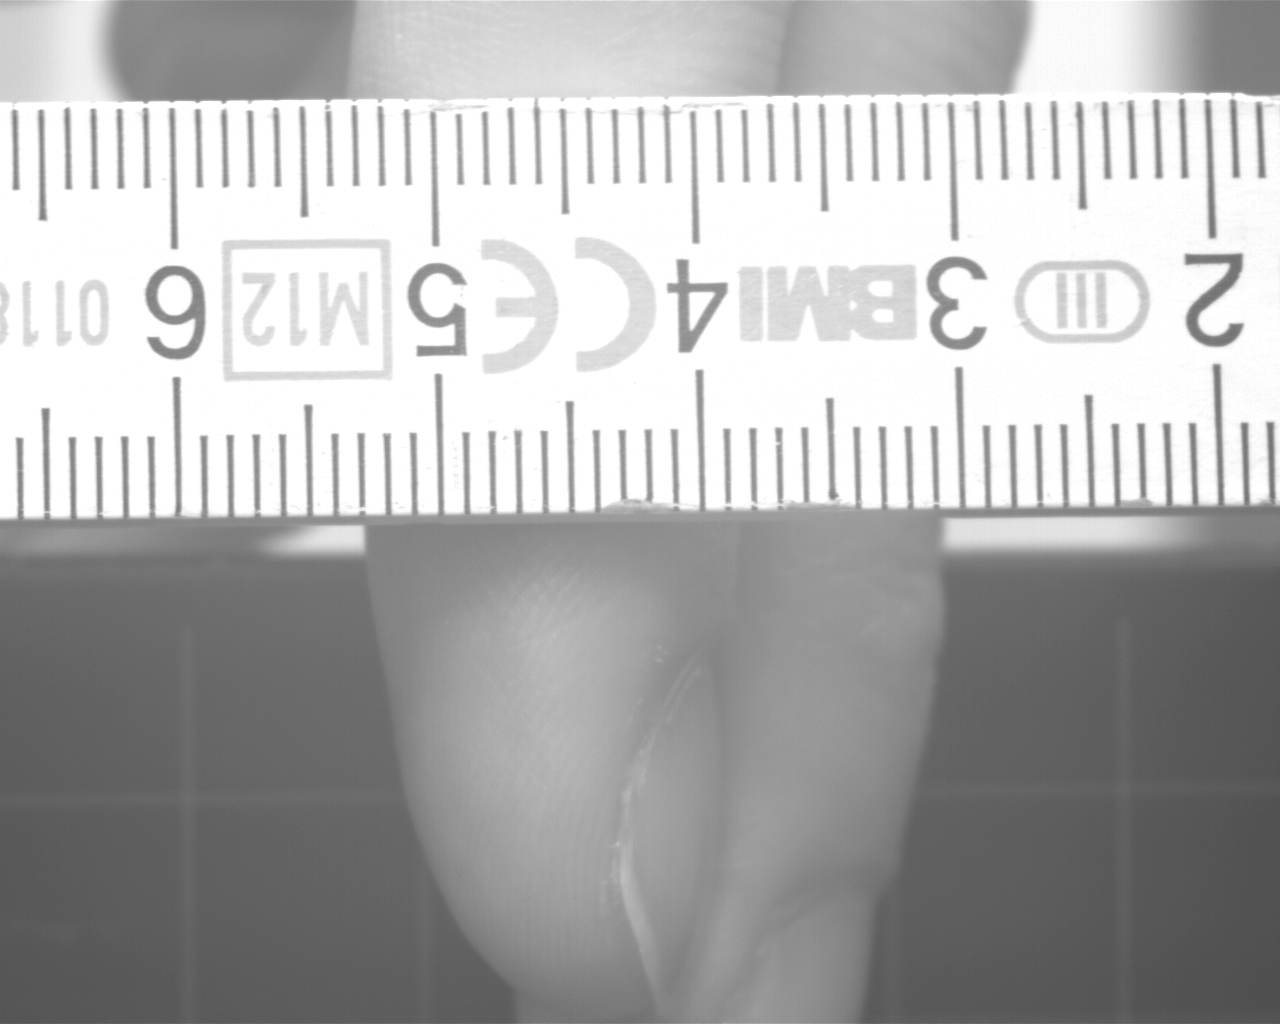
\includegraphics[width=\linewidth]{../Figures/scale.png}
        \caption{Millimeter scale at the same distance}
    \end{subfigure}
    \caption{Pictures to estimate the \mot's size.}
    \label{fig:mot_size}
\end{figure}

\subsection{Influence of quarter waveplates}

The effect of the $\lambda/4$ plates in front of the \mot{} have a significant
effect. This is shown in Figure~\ref{fig:lambda_front}. Depending on the
orientation of the plates the beam behind the plate stays linear or becomes
elliptic or circular polarized. This can suppress the formation of the
trap completely. The effect of the plates in the
backreflected beam can be seen in Figure~\ref{fig:lambda_behind}. It is not very
large. Ideally there should be no change of the \mot's power, of course.

\begin{figure}
    \centering
    \includegraphics[width=.7\textwidth]{lambda_front}
    \caption{%
        Effekt of the $\lambda/4$ plates in front of the vacuum chamber.
    }
    \label{fig:lambda_front}
\end{figure}

\begin{figure}
    \centering
    \includegraphics[width=.7\textwidth]{lambda_behind}
    \caption{%
        Effekt of the $\lambda/4$ plates behind the vacuum chamber.
    }
    \label{fig:lambda_behind}
\end{figure}

\subsection{Influence of magnetic field}

Go through the magnetic field current.

% TODO Tablet with magnetic field.

\subsection{Loading behaviour}

Pressure is supposed to be \SIrange{1.1e-7}{1.5e-7}{\milli\bar}

Room temperature \SI{24}{\celsius}

\subsection{Detuning of the laser frequencies}

Unlock the cooling laser. Run a slow frequency of around \SI{100}{\milli\hertz}
and scan the MOT intensity with the photo diode. 

\SI{3.9}{\milli\watt}

\end{document}

% vim: spell spelllang=en_us tw=79
